\documentclass[a4paper,landscape,12pt]{extarticle}
\usepackage[left=0.5in, right=0.5in, top=0.4in, bottom=0.55in]{geometry}
\usepackage{graphicx}
\usepackage[normalem]{ulem}
\usepackage{array}
\usepackage{caption}
\usepackage{amsmath}
\usepackage{fancyhdr}
\usepackage{lastpage}

\renewcommand\ULthickness{1.0pt}
\setlength\ULdepth{1.3ex}

\pagestyle{fancy}
\fancyhf{}
\renewcommand{\headrulewidth}{0pt}
\fancyfoot[R]{\Large\thepage\ / \pageref{LastPage}}

\newcommand{\slideheader}[2]{%
\noindent

\includegraphics[height=0.5in]{./unit03/slides/images/cpp_logo.png}%
\hspace{0.3in}%
{\Large \uline{#1 \hfill #2}}%
\par\vspace{0.4in}
}

\newcommand{\contentstart}{%
\leftskip 0.6in \rightskip 0.6in
}
\newcommand{\contentend}{%
\leftskip 0in \rightskip 0in
}

\newcommand{\bodytext}{\LARGE}

\begin{document}
\begin{huge}

%%%%%%%%%%%%%%%%%%%%%%%%%%%%%%%%%%%%%%%%
% Slide 1 - Title
\slideheader{ECE5110 Numerical Modeling}{Unit 03}

\vspace{0.7in}
\begin{center}
{\Huge \textbf{Three-Point Finite-Difference Differentiation}}\\[0.2in]
{\Large Plus Composite Trapezoidal and Simpson Integration}\\[0.6in]
{\Large Carson Quesada, Ishmael Taleo, Juan Ortiz,}\\
{\Large Michael Lanfranchi, Rushi Sharma, Timothy Jung}
\end{center}

%%%%%%%%%%%%%%%%%%%%%%%%%%%%%%%%%%%%%%%%
\newpage
\slideheader{Problem Overview}{Unit 03}
\contentstart
{\bodytext
\begin{itemize}
    \item Approximate first derivatives from sampled data using three-point stencils.
    \item Validate central, forward, and backward formulas against analytic derivatives.
    \item Validate composite trapezoidal and Simpson rules on an integral with exact value $\pi$.
    \item Apply the differentiation workflow to estimate $g$ from free-fall position-time measurements.
\end{itemize}
}
\contentend

%%%%%%%%%%%%%%%%%%%%%%%%%%%%%%%%%%%%%%%%
\newpage
\slideheader{Core Formulas}{Unit 03}
\contentstart
{\bodytext
\begin{itemize}
    \item Central:
    \[
    f'(x) \approx \frac{f(x+h)-f(x-h)}{2h}
    \]
    \item Forward:
    \[
    f'(x) \approx \frac{-3f(x)+4f(x+h)-f(x+2h)}{2h}
    \]
    \item Backward:
    \[
    f'(x) \approx \frac{f(x-2h)-4f(x-h)+3f(x)}{2h}
    \]
\end{itemize}
}
\contentend

%%%%%%%%%%%%%%%%%%%%%%%%%%%%%%%%%%%%%%%%
\newpage
\slideheader{Analytic Validation Results}{Unit 03}
\contentstart
{\bodytext
\begin{itemize}
    \item Test functions: $\sin(x)$ at $\pi/4$, $e^x$ at $0.3$, and $x^3-2x^2+x-5$ at $1.2$.
    \item Step size: $h=10^{-5}$.
    \item All 9 method-function combinations passed tolerance with errors below $1.5\times10^{-10}$.
\end{itemize}

\vspace{0.15in}
\begin{center}
\begin{tabular}{|l|c|c|}
\hline
Function and point & Method & Abs. error \\\hline
$\sin(\pi/4)$ & central & $1.40\times10^{-11}$ \\\hline
$e^{0.3}$ & forward & $3.38\times10^{-11}$ \\\hline
$p'(1.2)$ & backward & $1.40\times10^{-10}$ \\\hline
\end{tabular}
\end{center}
}
\contentend

%%%%%%%%%%%%%%%%%%%%%%%%%%%%%%%%%%%%%%%%
\newpage
\slideheader{Composite Integration Formulas}{Unit 03}
\contentstart
{\bodytext
\begin{itemize}
    \item Trapezoidal:
    \[
    \int_a^b f(x)\,dx \approx h\left[\frac{f(x_0)+f(x_n)}{2}+\sum_{i=1}^{n-1}f(x_i)\right]
    \]
    \item Simpson (even $n$):
    \[
    \int_a^b f(x)\,dx \approx \frac{h}{3}\left[f(x_0)+f(x_n)+4\sum_{i=1,\,\mathrm{odd}}^{n-1}f(x_i)+2\sum_{i=2,\,\mathrm{even}}^{n-2}f(x_i)\right]
    \]
    \item Benchmark integral:
    \[
    \int_0^1 \frac{4}{1+x^2}\,dx = \pi
    \]
\end{itemize}
}
\contentend

%%%%%%%%%%%%%%%%%%%%%%%%%%%%%%%%%%%%%%%%
\newpage
\slideheader{Integration Convergence Results}{Unit 03}
\contentstart
{\bodytext
\begin{itemize}
    \item Subinterval sweep: $n=4,8,16,32,64,128,256$ for both methods.
    \item Trapezoidal observed order: $1.99999$ (expected $2$).
    \item Simpson observed order: $6.65525$ (expected $4$; inflated by near-zero terminal errors).
    \item Finest-mesh errors: trapezoidal $2.543\times10^{-6}$, Simpson $0$ (within machine precision).
\end{itemize}

\vspace{0.15in}
\begin{center}
\begin{tabular}{|l|c|c|c|}
\hline
Method & Expected order & Observed order & Final tolerance pass \\\hline
Trapezoidal & 2 & 1.99999 & Yes \\\hline
Simpson & 4 & 6.65525 & Yes \\\hline
\end{tabular}
\end{center}
}
\contentend

%%%%%%%%%%%%%%%%%%%%%%%%%%%%%%%%%%%%%%%%
\newpage
\slideheader{Integration Error Plots}{Unit 03}
\contentstart
\begin{center}

\includegraphics[width=0.45\linewidth]{../results/plots/integration_trapezoidal_error_vs_h.png}
\hspace{0.03\linewidth}

\includegraphics[width=0.45\linewidth]{../results/plots/integration_simpson_error_vs_h.png}
\captionof{figure}{Log-log absolute error trends for composite trapezoidal and Simpson rules on the $\pi$ benchmark.}
\end{center}
\contentend

%%%%%%%%%%%%%%%%%%%%%%%%%%%%%%%%%%%%%%%%
\newpage
\slideheader{Free-Fall Application}{Unit 03}
\contentstart
{\bodytext
\begin{itemize}
    \item Fit a quadratic interpolant to 7 measured position-time samples.
    \item Differentiate numerically twice using the central stencil.
    \item Evaluate at $t_0=0.174306\,\mathrm{s}$ to recover acceleration.
\end{itemize}
}

\vspace{0.1in}
\begin{center}
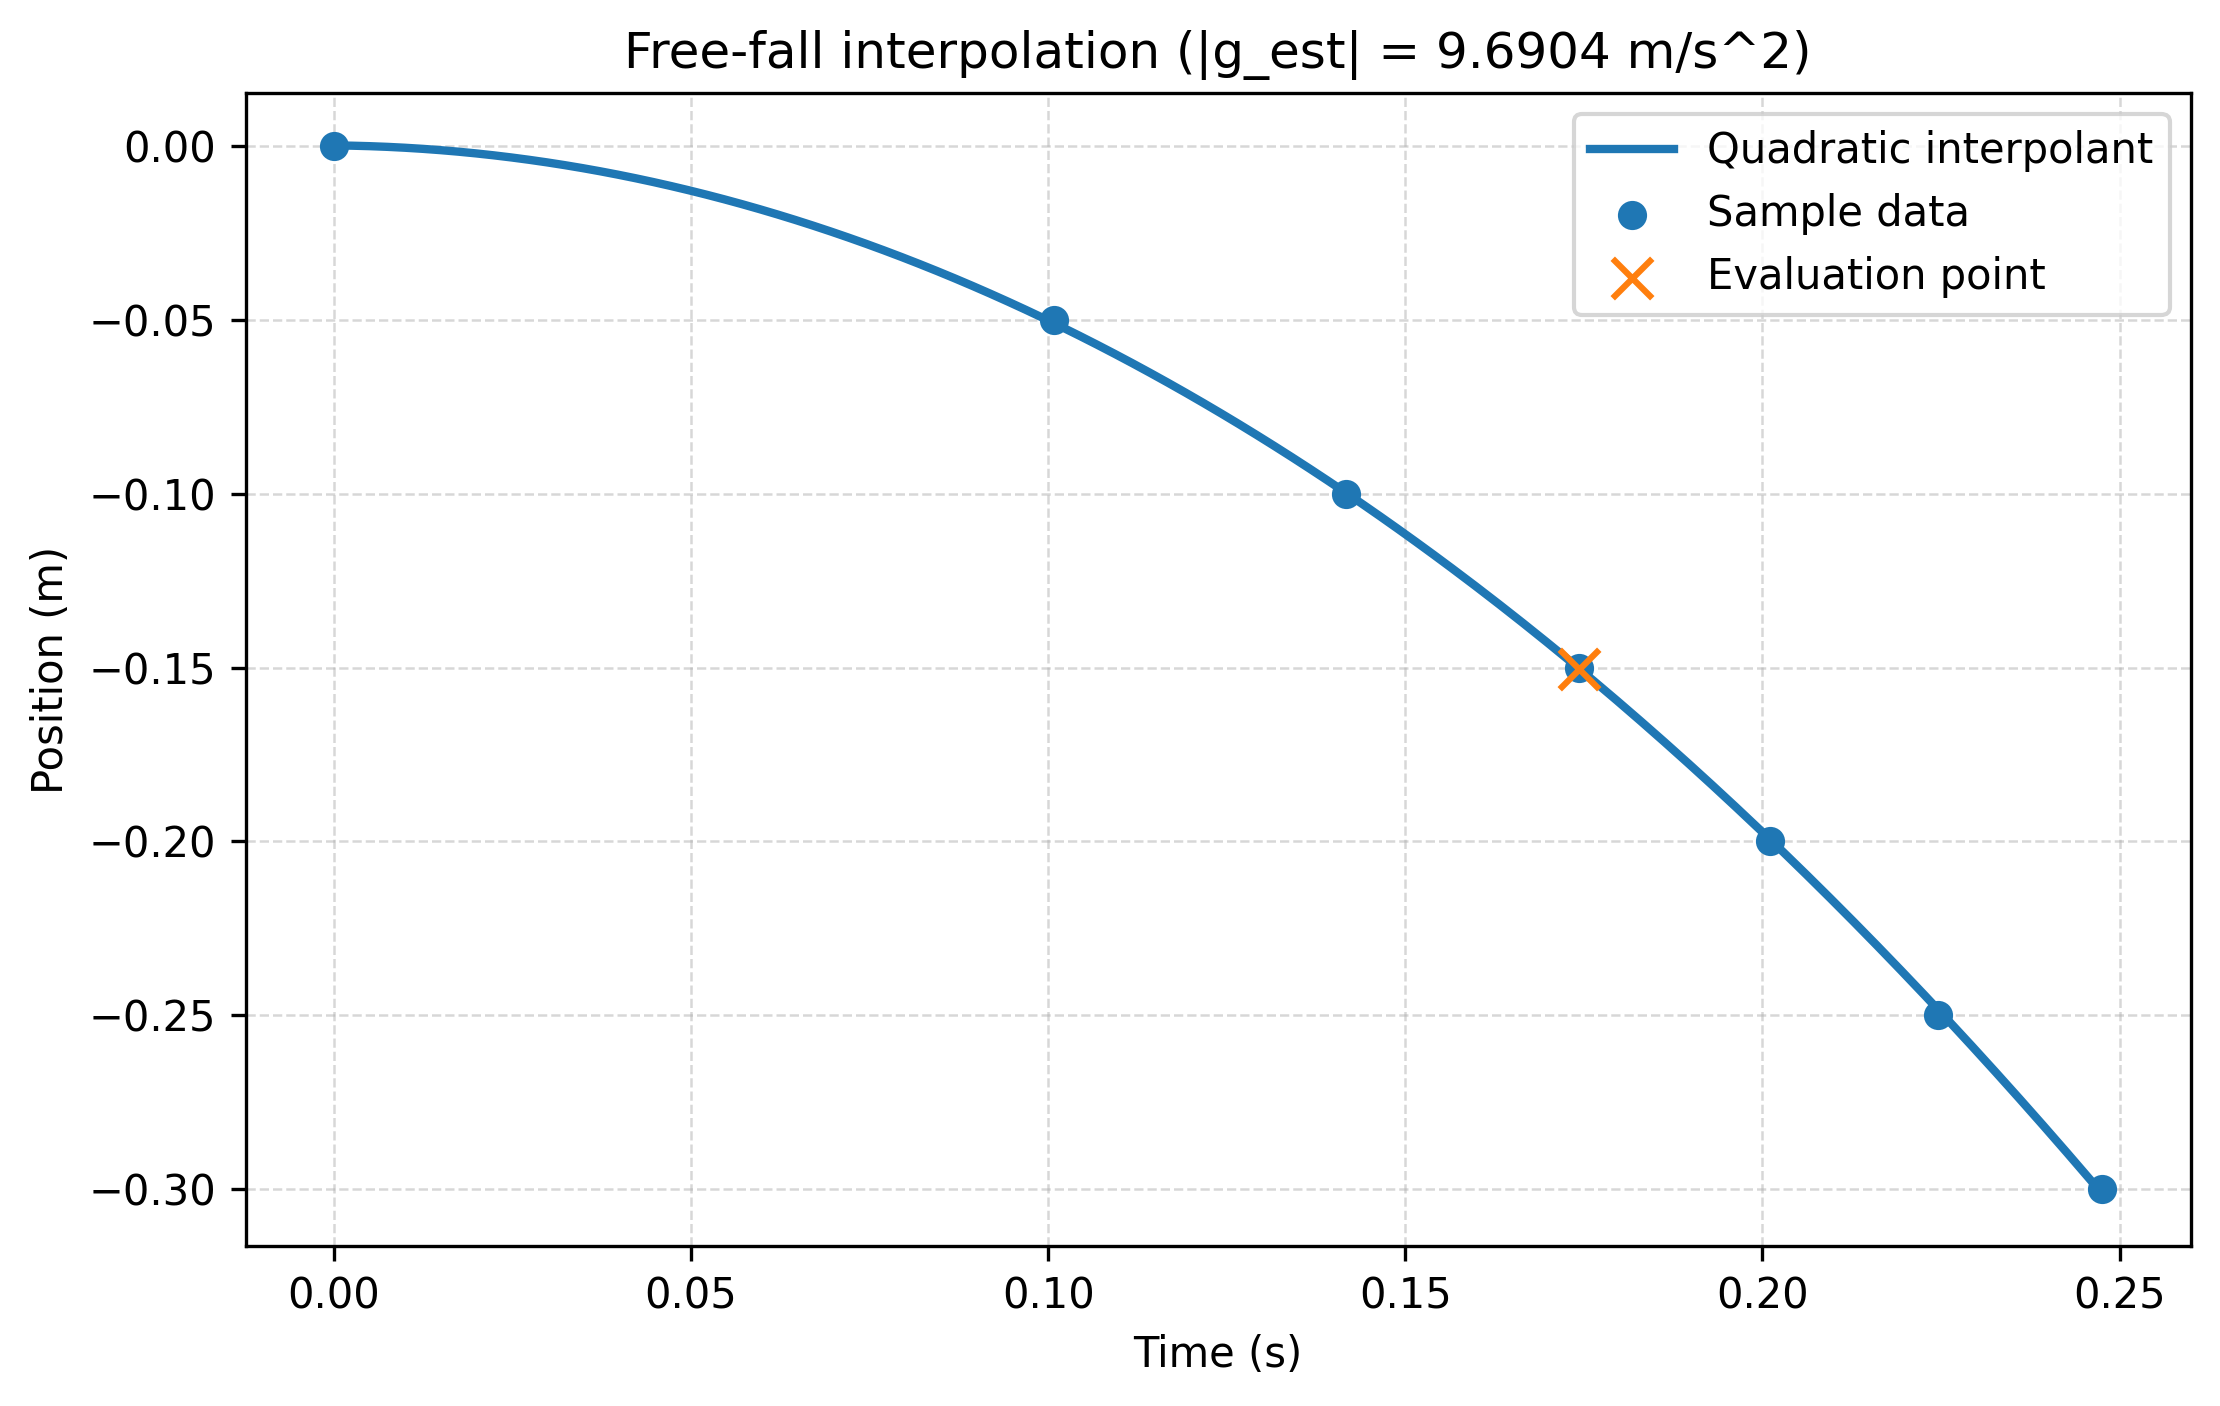
\includegraphics[width=0.73\linewidth]{../results/plots/freefall_gravity_interpolation.png}
\captionof{figure}{Quadratic interpolant fitted to measured free-fall data.}
\end{center}
\contentend

%%%%%%%%%%%%%%%%%%%%%%%%%%%%%%%%%%%%%%%%
\newpage
\slideheader{Estimated Gravity}{Unit 03}
\contentstart
{\bodytext
\begin{itemize}
    \item Signed estimate: $\hat{a}=-9.6904\,\mathrm{m/s^2}$ (downward direction).
    \item Magnitude: $|\hat{g}|=9.6904\,\mathrm{m/s^2}$.
    \item Reference: $9.81\,\mathrm{m/s^2}$.
    \item Absolute magnitude error: $0.1196\,\mathrm{m/s^2}$.
    \item Tolerance check: pass ($0.1196 < 0.15$).
\end{itemize}
}
\contentend

%%%%%%%%%%%%%%%%%%%%%%%%%%%%%%%%%%%%%%%%
\newpage
\slideheader{Repository Skills (Numerical Workflows)}{Unit 03}
\contentstart
{\bodytext
\begin{itemize}
    \item \textbf{differentiation-3point}: Builds and validates 3-point finite-difference workflows, exports CSV/JSON/Markdown outputs, generates plots, and estimates free-fall gravity.
    \item \textbf{integration-trapezoidal}: Implements composite trapezoidal integration with benchmark tests, convergence checks, and report-ready exports.
    \item \textbf{integration-simpson}: Implements composite Simpson integration with even-subinterval validation, fourth-order convergence analysis, and exported artifacts.
\end{itemize}
}
\contentend

%%%%%%%%%%%%%%%%%%%%%%%%%%%%%%%%%%%%%%%%
\newpage
\slideheader{Repository Skills (LaTeX and Presentation)}{Unit 03}
\contentstart
{\bodytext
\begin{itemize}
    \item \textbf{latex-article}: Generates IS\&T-style technical articles from a target subject using the course template and required structure.
    \item \textbf{latex-slides}: Builds concise unit slide decks by summarizing the corresponding article and reusing unit result figures.
    \item These skills standardize file locations, output artifacts, and formatting so results remain reproducible across assignments.
\end{itemize}
}
\contentend

%%%%%%%%%%%%%%%%%%%%%%%%%%%%%%%%%%%%%%%%
\newpage
\slideheader{Agents in This Repository}{Unit 03}
\contentstart
{\bodytext
\begin{itemize}
    \item Agents are specialized assistants configured in \texttt{.github/agents/}.
    \item They apply focused instructions, tools, and constraints for different task types.
    \item In this project, one agent is centered on LaTeX formatting and one on Python numerical workflows.
\end{itemize}
}
\contentend

%%%%%%%%%%%%%%%%%%%%%%%%%%%%%%%%%%%%%%%%
\newpage
\slideheader{Agent Summaries}{Unit 03}
\contentstart
{\bodytext
\begin{itemize}
    \item \textbf{ECE5110 LaTeX Formatter Agent}: Maintains consistent article/slide structure, styling, and build integrity; follows course templates and formatting constraints.
    \item \textbf{ECE5110 Python Numerical Agent}: Implements and validates numerical methods in \texttt{lib/} and \texttt{unit03/test/}, produces reproducible result artifacts and plots.
    \item Combined workflow: skills define reusable task recipes, while agents enforce role-specific quality and project conventions.
\end{itemize}
}
\contentend

%%%%%%%%%%%%%%%%%%%%%%%%%%%%%%%%%%%%%%%%
\newpage
\slideheader{Conclusions}{Unit 03}
\contentstart
{\bodytext
\begin{itemize}
    \item Three-point finite-difference methods achieved strong analytic accuracy.
    \item Central differencing provided the best overall error performance.
    \item Trapezoidal and Simpson integration both passed convergence and final-accuracy checks.
    \item Simpson reached near machine precision on the smooth benchmark integral.
    \item Interpolation plus numerical differentiation recovered $g$ within 1.2\% of the standard value.
\end{itemize}
}
\contentend

%%%%%%%%%%%%%%%%%%%%%%%%%%%%%%%%%%%%%%%%
\newpage
\slideheader{Unit 03}{ECE5110 - Numerical Modeling}
\vspace{2.5in}
\begin{center}
{\Huge \textbf{Questions?}}
\end{center}

\end{huge}
\end{document}
